\documentclass{beamer}
\usetheme{metropolis}
\usecolortheme{spruce}
\usepackage{amsmath}
\usepackage{graphicx}
\usepackage{booktabs}
\usepackage{caption}
\usepackage{listings}
\lstset{
	basicstyle=\ttfamily\tiny, % Adjusted for richer content
	breaklines=true,
	frame=single,
	numbers=left,
	numberstyle=\tiny\color{gray},
	backgroundcolor=\color{gray!10},
	keywordstyle=\color{blue},
	stringstyle=\color{red},
	commentstyle=\color{green!60!black},
	language=R % Default, switches to Python
}

% Title slide information
\title{Regression \& Prediction}
\subtitle{Theory and Practice with House Prices}
\author{Your Name}
\institute{xAI}
\date{February 23, 2025}

\begin{document}
	
	% Title Slide
	\begin{frame}
		\titlepage
	\end{frame}
	
	% Outline Slide
	\begin{frame}{Our Housing Journey}
		\begin{columns}
			\column{0.5\textwidth}
			\begin{itemize}
				\item Starting Simple: Foundations
				\item Expanding the Scope: Complexity
				\item Refining Precision: Optimization
			\end{itemize}
			\column{0.5\textwidth}
			\begin{itemize}
				\item Facing Challenges: Pitfalls
				\item Insights \& Next Steps: Applications
			\end{itemize}
		\end{columns}
		\metroset{block=fill}
		\begin{block}{Focus}
			Unpacking King County house prices with rich theory and dual R/Python implementations
		\end{block}
	\end{frame}
	
	% Outline Slide
	\begin{frame}{The Quest to Understand Relationships}
		\begin{itemize}
			\item Imagine you are exploring data to understand how different factors relate to each other.
			\item That’s regression: a tool to ask, ``How does $Y$ change with $X$, and can we predict it?''
			\item In very basically It’s the bridge between stats, where we explain the past, and data science, where we predict the future—our journey begins here.
		\end{itemize}
	\end{frame}
	
	
	% Section 1: Starting Simple
	\section{Starting Simple}
	
	\begin{frame}{The Housing Puzzle}
		\begin{itemize}
			\item \textbf{Objective}: Decode drivers of house prices in King County—size, location, features
			\item \textbf{Regression}: A statistical lens linking price ($Y$) to predictors like size ($X$)
			\item \textbf{Purpose}: Explain historical sales patterns and forecast future values for buyers and assessors
		\end{itemize}
	\end{frame}
	
	\begin{frame}[fragile]{Simple Linear Regression: Theory \& R}
		\begin{columns}
			\column{0.6\textwidth}
			\begin{itemize}
				\item \textbf{Theory}: Models a straight-line relationship: $Y = b_0 + b_1X + e$
				\item $b_0$: Base price when size is zero; $b_1$: Price increase per sq ft; $e$: Random error
				\item Assumes linearity and independence—foundation of regression
			\end{itemize}
			\begin{lstlisting}
# R 
simple_lm <- lm(AdjSalePrice ~ SqFtTotLiving, data = house_df)
# Create the plot
ggplot(house_df, aes(x = sqft_living, y = price)) +
geom_point(alpha = 0.5) +  # Scatter plot
geom_smooth(method = "lm", color = "blue", se = FALSE) +  # Regression line
labs(title = "Price vs. Size Fit",
x = "Size (sqft_living)",
y = "Price") +
theme_minimal()
# Output: Coefficients:
(Intercept)  sqft_living  
-43580.7        280.6 

			\end{lstlisting}
			\column{0.4\textwidth}
		\begin{figure}
			\centering
			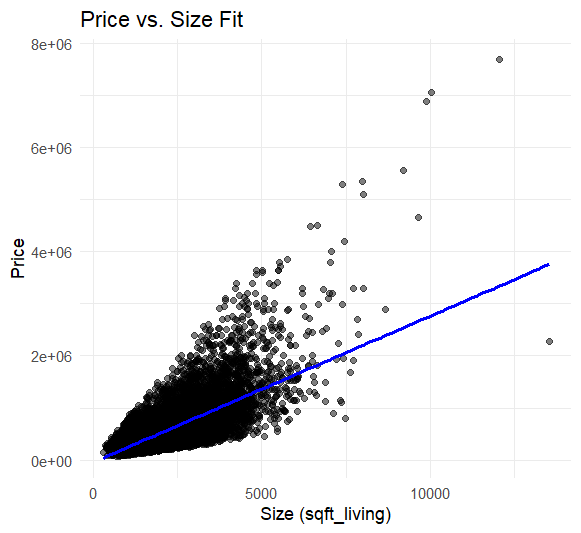
\includegraphics[width=\textwidth]{regres1.jpg} % Use .png, .jpg, or .jpeg instead of .pdf
			\caption{Price vs. Size Fit}
			\label{fig:price_vs_size_fit}
			\begin{itemize}
				\item Size as a core driver
			\end{itemize}
			\begin{itemize}
				\item b0=−43580.7 , b1=280.6
			\end{itemize}
		\end{figure}
		\end{columns}
	\end{frame}
	
	\begin{frame}[fragile]{Simple Linear Regression: Python}
		\lstset{language=Python}
		\begin{columns}
			\column{0.6\textwidth}
			\begin{itemize}
				\item \textbf{Practice}: Fits price to living space, revealing size’s impact
				\item \textbf{Key Insight}: Positive slope shows larger homes fetch higher prices
			\end{itemize}
			\begin{lstlisting}
# Python (p. 152 adapted)
from sklearn.linear_model import LinearRegression
predictors = ['SqFtTotLiving']
outcome = 'AdjSalePrice'
simple_lm = LinearRegression()
simple_lm.fit(house[predictors], house[outcome])
# Example: Intercept ~ base, Coef ~ $ per sq ft
			\end{lstlisting}
			\column{0.4\textwidth}

		\end{columns}
	\end{frame}
	
	\begin{frame}{Finding the Best Fit: Least Squares}
			\begin{itemize}
				 \item \textbf{How do we draw that line?} We minimize the mess—sum of squared errors
				\item \textbf{Theory}: Finds the line minimizing residual sum of squares: $\sum_{i=1}^n (Y_i - \hat{Y}_i)^2$
				\item \textbf{How}: Adjusts $b_0$ and $b_1$ to reduce prediction errors—optimal for linear fits
				\item \textbf{History}: Legendre (1805) and Gauss; computationally efficient but outlier-sensitive in small datasets
			\end{itemize}
		\end{frame}
		
		\begin{frame}[fragile]{Finding the Best Fit: Least Squares}
		\lstset{language=Python}
\begin{columns}
	\column{0.9\textwidth}
			\begin{lstlisting}
Coefficients:
Estimate Std. Error t value Pr(>|t|)    
(Intercept) -5.957e+05  1.325e+04 -44.950  < 2e-16 ***
sqft_living  2.065e+02  3.364e+00  61.373  < 2e-16 ***
sqft_lot    -2.664e-01  4.171e-02  -6.388 1.71e-10 ***
bathrooms   -3.944e+04  3.443e+03 -11.456  < 2e-16 ***
grade        1.037e+05  2.285e+03  45.379  < 2e-16 ***
---
Signif. codes:  0 ‘***’ 0.001 ‘**’ 0.01 ‘*’ 0.05 ‘.’ 0.1 ‘ ’ 1

Residual standard error: 249600 on 21608 degrees of freedom
Multiple R-squared:  0.538,	Adjusted R-squared:  0.5379 
F-statistic:  6291 on 4 and 21608 DF,  p-value: < 2.2e-16
		\end{lstlisting}
				
			\begin{lstlisting}
# R
summary(house_lm)# Model Summary (Extracts Coefficients, p-values, R²)
predictions <- predict(house_lm, newdata = house_df)# Extract RMSE
residuals <- house_df$price - predictions
RMSE <- sqrt(mean(residuals^2))
R_squared <- summary(house_lm)$r.squared # Extract R-squared
p_values <- summary(house_lm)$coefficients[, 4] # Extract P-values
# Print Results
cat("RMSE:", RMSE, "\n")
cat("R²:", R_squared, "\n")
cat("P-values:\n")
print(p_values)
			\end{lstlisting}
			\column{0.4\textwidth}
			
		\end{columns}
	\end{frame}


	
	
	% Section 2: Expanding the Scope
	\section{Expanding the Scope}
	
	\begin{frame}[fragile]{More Clues: Multiple Linear Regression}
		\begin{columns}
			\column{0.6\textwidth}
			\begin{itemize}
				\item \textbf{Theory}: Extends to multiple predictors: $Y = b_0 + b_1X_1 + b_2X_2 + \dots + e$
				\item \textbf{Power}: Captures combined effects—size, lot, bedrooms—assuming linearity
				\item \textbf{Use}: Explains complex housing dynamics
			\end{itemize}
			\begin{lstlisting}
# R (p. 152)
house_lm <- lm(AdjSalePrice ~ SqFtTotLiving + SqFtLot + Bathrooms +
Bedrooms + BldgGrade, data = house)
# Coefs: SqFtTotLiving = 228.831, Bedrooms = -47769.955
			\end{lstlisting}
			\column{0.4\textwidth}
			\begin{itemize}
				\item Size adds \$229/sq ft
			\end{itemize}
		\end{columns}
	\end{frame}
	

% Section 2: Key Findings

\begin{frame}[fragile]{Multiple Linear Regression: Key Findings}
	\begin{columns}
		\column{0.9\textwidth}
		\begin{lstlisting}
lm(formula = price ~ sqft_living + sqft_lot + bathrooms + bathrooms + 
grade, data = house_df, na.action = na.omit)

Coefficients:
(Intercept)  sqft_living     sqft_lot    bathrooms        grade  
-5.957e+05    2.065e+02   -2.664e-01   -3.944e+04    1.037e+05  
		\end{lstlisting}
		\begin{itemize}
			\item \textbf{sqft\_living}: 🏡 +\$206.5 per sq ft → Larger houses increase price significantly.
			\item \textbf{grade}: 🔼 +\$103,700 per unit → Higher quality homes boost price.
			\item \textbf{sqft\_lot}: 🌲 -\$0.266 per sq ft → Lot size has a tiny negative effect.
			\item \textbf{bathrooms}: 🚿 -\$39,440 per extra bathroom → Unexpected negative impact.
		\end{itemize}
	\end{columns}
\end{frame}


% Section 3: Model Performance
\begin{frame}[fragile]{Multiple Linear Regression:Model Evaluation}
	\begin{columns}
		\column{0.9\textwidth}
		\begin{lstlisting}
> cat("RMSE:", RMSE, "\n")
RMSE: 249532.2 
> cat("R²:", R_squared, "\n")
R²: 0.5380018 
> cat("P-values:\n")
P-values:
		\end{lstlisting}
		\begin{itemize}
			\item \textbf{RMSE}: 📉 $261,300 → Predictions are off by ~$261K on average.
			\item \textbf{$R^2$}: 📊 0.5406 (54.06%) → The model explains 54% of price variation..
			\item \textbf{P-values}: 🧪 SqFtLot is **not statistically significant (p = 0.323)`
		\end{itemize}
	\end{columns}
\end{frame}

	
	\begin{frame}[fragile]{Multiple Linear Regression: Python}
		\lstset{language=Python}
		\begin{columns}
			\column{0.6\textwidth}
			\begin{itemize}
				\item \textbf{Practice}: Models housing with multiple factors
				\item \textbf{Key Insight}: Negative bedroom coef suggests smaller rooms hurt value
			\end{itemize}
			\begin{lstlisting}
# Define predictors and outcome
predictors = ['sqft_living', 'sqft_lot', 'bathrooms', 'grade']
outcome = 'price'

# Fit Multiple Linear Regression Model
house_lm = LinearRegression()
house_lm.fit(house_df[predictors], house_df[outcome])

			\end{lstlisting}
			\column{0.4\textwidth}
			\begin{itemize}
				\item Bedrooms vs. size tension
			\end{itemize}
		\end{columns}
	\end{frame}
	
	% Section 2: Expanding the Scope
	\begin{frame}[fragile]{Factor Variables: Theory \& R}
		\begin{columns}
			\column{0.6\textwidth}
			\begin{itemize}
				\item \textbf{Theory (p. 163)}: Encodes categorical variables (e.g., property type) as binary dummies
				\item \textbf{Why}: Allows non-numeric factors in regression; compares to a reference level
				\item \textbf{Example}: Single-family vs. Townhouse effects
			\end{itemize}
			\begin{lstlisting}
# R (p. 164)
prop_type_dummies <- model.matrix(~ PropertyType - 1, data = house)
# Output: 1 for each type present
			\end{lstlisting}
			\column{0.4\textwidth}
			\begin{itemize}
				\item Type shifts price
			\end{itemize}
		\end{columns}
	\end{frame}
	
	\begin{frame}[fragile]{Factor Variables: Python}
		\lstset{language=Python}
		\begin{columns}
			\column{0.6\textwidth}
			\begin{itemize}
				\item \textbf{Practice}: Integrates property type into price model
				\item \textbf{Key Insight}: Townhouses may differ from single-family homes
			\end{itemize}
			\begin{lstlisting}
# Python (p. 166 adapted)
import pandas as pd
X = pd.get_dummies(house['PropertyType'], drop_first=True)
# Drops first level (e.g., Multiplex) as reference
			\end{lstlisting}
			\column{0.4\textwidth}
			\begin{itemize}
				\item Baseline comparison
			\end{itemize}
		\end{columns}
	\end{frame}
	
	\begin{frame}[fragile]{Nonlinear Fit: Theory \& Splines in R}
		\begin{columns}
			\column{0.6\textwidth}
			\begin{itemize}
				\item \textbf{Theory (p. 187)}: Nonlinear via polynomial segments joined at knots
				\item \textbf{Why}: Captures diminishing returns—e.g., small homes gain more per sq ft
				\item \textbf{Advantage}: Flexible fit without overfitting like high-order polynomials
			\end{itemize}
			\begin{lstlisting}
# R (p. 190)
library(splines)
knots <- quantile(house_98105$SqFtTotLiving, p = c(.25, .5, .75))
lm_spline <- lm(AdjSalePrice ~ bs(SqFtTotLiving, knots = knots, degree = 3) +
SqFtLot + Bathrooms + Bedrooms + BldgGrade, data = house_98105)
			\end{lstlisting}
			\column{0.4\textwidth}
			\begin{figure}
				\includegraphics[width=\textwidth]{figure4-12-placeholder.pdf}
				\caption{Spline Fit}
			\end{figure}
		\end{columns}
	\end{frame}
	
	\begin{frame}[fragile]{Nonlinear Fit: Splines in Python}
		\lstset{language=Python}
		\begin{columns}
			\column{0.6\textwidth}
			\begin{itemize}
				\item \textbf{Practice}: Fits nonlinear price trends in zip 98105
				\item \textbf{Key Insight}: Better matches small vs. large home value shifts
			\end{itemize}
			\begin{lstlisting}
# Python (p. 190)
import statsmodels.formula.api as smf
formula = 'AdjSalePrice ~ bs(SqFtTotLiving, df=6, degree=3) + SqFtLot + Bathrooms + Bedrooms + BldgGrade'
model_spline = smf.ols(formula=formula, data=house_98105).fit()
			\end{lstlisting}
			\column{0.4\textwidth}
			\begin{itemize}
				\item Curves reflect reality
			\end{itemize}
		\end{columns}
	\end{frame}

	
	

	
	% Section 3: Refining Precision
	\section{Refining Precision}
	
	

	
	\begin{frame}{Model Assessment: Theory}
		\begin{itemize}
			\item \textbf{Theory (p. 153)}: Measures prediction quality and fit
			\item \textbf{RMSE}: $\sqrt{\frac{\sum (y_i - \hat{y}_i)^2}{n}}$—average error magnitude
			\item \textbf{$R^2$}: Proportion of variance explained (0-1); higher means better fit
			\item \textbf{Use}: Guides housing prediction accuracy
		\end{itemize}
	\end{frame}
	
	\begin{frame}{Cross-Validation: Theory}
		\begin{itemize}
			\item \textbf{Theory (p. 155)}: Validates model on unseen data via $k$-fold splits
			\item \textbf{Process}: Divide data, train on $k-1$, test on 1, repeat, average RMSE
			\item \textbf{Why}: Ensures predictions generalize beyond training sales—crucial for real estate
		\end{itemize}
	\end{frame}
	
	\begin{frame}[fragile]{Model Selection: Theory \& R}
		\begin{columns}
			\column{0.6\textwidth}
			\begin{itemize}
				\item \textbf{Theory (p. 156)}: Balances fit vs. complexity—Occam’s razor
				\item \textbf{AIC}: $2P + n\log(\text{RSS}/n)$—penalizes extra predictors
				\item \textbf{Goal}: Optimal housing model without overkill
			\end{itemize}
			\begin{lstlisting}
# R (p. 157)
library(MASS)
house_full <- lm(AdjSalePrice ~ SqFtTotLiving + SqFtLot + Bathrooms +
Bedrooms + BldgGrade + PropertyType, data = house)
step <- stepAIC(house_full, direction = "both")
# Drops less impactful vars
			\end{lstlisting}
			\column{0.4\textwidth}
			\begin{itemize}
				\item Streamlined predictors
			\end{itemize}
		\end{columns}
	\end{frame}
	
	\begin{frame}[fragile]{Model Selection: Python}
		\lstset{language=Python}
		\begin{columns}
			\column{0.6\textwidth}
			\begin{itemize}
				\item \textbf{Practice}: Automates predictor choice for housing
				\item \textbf{Key Insight}: Reduces noise, enhances prediction
			\end{itemize}
			\begin{lstlisting}
# Python (p. 158 adapted)
from dmba import stepwise_selection
predictors = ['SqFtTotLiving', 'SqFtLot', 'Bathrooms', 'Bedrooms', 'BldgGrade']
def train_model(vars):
model = LinearRegression()
model.fit(house[vars], house[outcome])
return model
best_model, _ = stepwise_selection(house[predictors].columns, train_model)
			\end{lstlisting}
			\column{0.4\textwidth}
			\begin{itemize}
				\item Focused fit
			\end{itemize}
		\end{columns}
	\end{frame}
	
	\begin{frame}[fragile]{Weighted Regression: Theory \& R}
		\begin{columns}
			\column{0.6\textwidth}
			\begin{itemize}
				\item \textbf{Theory (p. 159)}: Weights adjust influence by reliability
				\item \textbf{Why}: Older sales less relevant—recent data gets priority
				\item \textbf{Impact}: Refines coefficients for current market
			\end{itemize}
			\begin{lstlisting}
# R (p. 159)
house$Weight = year(house$DocumentDate) - 2005
house_wt <- lm(AdjSalePrice ~ SqFtTotLiving + SqFtLot + Bathrooms +
Bedrooms + BldgGrade, data = house, weight = Weight)
# Shifts coefs slightly
			\end{lstlisting}
			\column{0.4\textwidth}
			\begin{itemize}
				\item Recent sales emphasized
			\end{itemize}
		\end{columns}
	\end{frame}
	
	\begin{frame}[fragile]{Weighted Regression: Python}
		\lstset{language=Python}
		\begin{columns}
			\column{0.6\textwidth}
			\begin{itemize}
				\item \textbf{Practice}: Weights tune housing model
				\item \textbf{Key Insight}: Aligns predictions with market trends
			\end{itemize}
			\begin{lstlisting}
# Python (p. 160)
house['Weight'] = [int(date.split('-')[0]) for date in house.DocumentDate] - 2005
house_wt = LinearRegression()
house_wt.fit(house[predictors], house[outcome], sample_weight=house.Weight)
			\end{lstlisting}
			\column{0.4\textwidth}
			\begin{itemize}
				\item Fresher focus
			\end{itemize}
		\end{columns}
	\end{frame}
	
	% Section 4: Facing Challenges
	\section{Facing Challenges}
	
	\begin{frame}{Prediction Limits: Theory}
		\begin{itemize}
			\item \textbf{Theory (p. 161)}: Extrapolation beyond data fails—e.g., empty lots
			\item \textbf{Intervals}: Confidence for $b_i$, wider prediction for $\hat{Y}_i$
			\item \textbf{Why}: Uncertainty spikes outside training range—limits housing forecasts
		\end{itemize}
	\end{frame}
	
	\begin{frame}{Interpreting Coefficients: Theory}
		\begin{itemize}
			\item \textbf{Theory (p. 171)}: Coefficients mislead if predictors correlate
			\item \textbf{Multicollinearity}: Size and bedrooms overlap—unstable fits
			\item \textbf{Confounding}: Missing location skews results
			\item \textbf{Interactions}: Size’s effect varies by zip—needs modeling
		\end{itemize}
	\end{frame}
	
	\begin{frame}[fragile]{Diagnostics: Theory \& R}
		\begin{columns}
			\column{0.6\textwidth}
			\begin{itemize}
				\item \textbf{Theory (p. 176)}: Residuals reveal model flaws
				\item \textbf{Outliers}: Extreme sales (e.g., \$119,748); \textbf{Influence}: Sway points
				\item \textbf{Heteroskedasticity}: Uneven errors signal gaps
			\end{itemize}
			\begin{lstlisting}
# R (p. 177)
house_98105 <- house[house$ZipCode == 98105, ]
lm_98105 <- lm(AdjSalePrice ~ SqFtTotLiving + SqFtLot + Bathrooms +
Bedrooms + BldgGrade, data = house_98105)
sresid <- rstandard(lm_98105)  # -4.326732 outlier
			\end{lstlisting}
			\column{0.4\textwidth}
			\begin{figure}
				\includegraphics[width=\textwidth]{figure4-6-placeholder.pdf}
				\caption{Influence Plot}
			\end{figure}
		\end{columns}
	\end{frame}
	
	\begin{frame}[fragile]{Diagnostics: Python}
		\lstset{language=Python}
		\begin{columns}
			\column{0.6\textwidth}
			\begin{itemize}
				\item \textbf{Practice}: Identifies \$119,748 as partial sale anomaly
				\item \textbf{Key Insight}: Diagnostics ensure robust housing predictions
			\end{itemize}
			\begin{lstlisting}
# Python (p. 178)
from statsmodels.stats.outliers_influence import OLSInfluence
house_98105 = house[house['ZipCode'] == 98105]
model = smf.ols('AdjSalePrice ~ SqFtTotLiving + SqFtLot + Bathrooms + Bedrooms + BldgGrade', data=house_98105).fit()
influence = OLSInfluence(model)
sresiduals = influence.resid_studentized
			\end{lstlisting}
			\column{0.4\textwidth}
			\begin{itemize}
				\item Spots critical flaws
			\end{itemize}
		\end{columns}
	\end{frame}
	
	\begin{frame}[fragile]{Influence Plot (Bubble Plot) – Identify Influential Values}
		\begin{itemize}
			\item \textbf{Purpose:} Identifies influential observations by combining leverage, residuals, and Cook’s Distance.
			\item \textbf{Key Insights:}
			\begin{itemize}
				\item Large bubbles = high Cook’s Distance → Removing these changes regression results significantly.
				\item Possible reasons:
				\begin{enumerate}
					\item High leverage (extreme predictor values) , Large residual (far from regression line) ,Both high leverage and large residual.
				\end{enumerate}
			\end{itemize}
			\item \textbf{Results:} Four large influential points found (Cook’s D > 0.08), impacting coefficients.
			\item Residuals beyond ±2.5
		\end{itemize}
		

	\end{frame}
	
	
	\begin{frame}[fragile]{Influence Plot (Bubble Plot) – Identify Influential Values}
		\begin{columns}
		
			\column{0.8\textwidth}
			\begin{figure}
				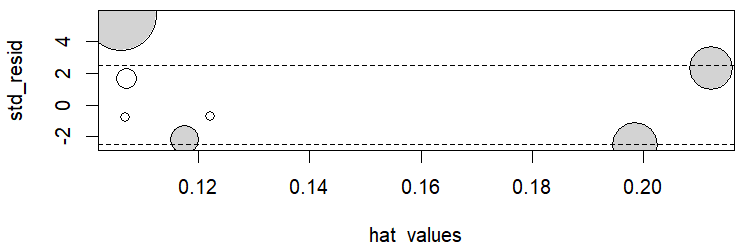
\includegraphics[width=0.8\textwidth]{influence_plot.png}
				\caption{Bubble plot showing influential points.}
			\end{figure}
		\end{columns}
	\end{frame}
	
	\begin{frame}[fragile]{Influence Plot (Bubble Plot) – Identify Influential Values}
		\begin{itemize}
		\end{itemize}

				\begin{lstlisting}[language=R, caption=Influence Plot in R]
library(car)
lm_model <- lm(AdjSalePrice ~ SqFtTotLiving + SqFtLot + Bathrooms + Bedrooms + BldgGrade, data=house_98105)
influencePlot(lm_model)
		\end{lstlisting}
		\begin{lstlisting}[language=Python, caption=Influence Plot in Python]
house_98105 = house[house['ZipCode'] == 98105]
X = house_98105[['SqFtTotLiving', 'SqFtLot', 'Bathrooms', 'Bedrooms', 'BldgGrade']].assign(const=1)
y = house_98105['AdjSalePrice']
model = sm.OLS(y, X).fit()
influence = sm.stats.outliers_influence.OLSInfluence(model)
fig, ax = plt.subplots(figsize=(5, 5))
ax.axhline(-2.5, ls='--', color='C1')
ax.axhline(2.5, ls='--', color='C1')
ax.scatter(influence.hat_matrix_diag, influence.resid_studentized_internal,
s=1000 * np.sqrt(influence.cooks_distance[0]), alpha=0.5)
ax.set_xlabel('hat values')
ax.set_ylabel('studentized residuals')
plt.show()\
		\end{lstlisting}
	\end{frame}
	
		\begin{frame}{Residual Plot (Heteroskedasticity Check)}
		\begin{itemize}
			\item \textbf{Purpose:} The residual plot checks for heteroskedasticity by analyzing how residuals (errors) vary with predicted values.
			\item \textbf{Key Insights:}
			\begin{itemize}
				\item X-axis (Predicted Values): Represents the fitted values from the regression model.
				\item Y-axis (Absolute Residuals): Measures the deviation of actual values from predictions.
				\item Scatter Points: Each dot represents an observation’s residual.
				\item LOESS Smoother (Blue Line): Shows the trend in residuals.
				\item Shaded Region: Indicates confidence around the trend.
				\begin{enumerate}
					\item Heteroskedasticity detected – Residuals increase with larger predicted values, indicating variance instability.
					\item  Curved Trend – Suggests missing variables or non-linearity in the data.
					\item Outliers at High Predictions – Some extreme points have large residuals, further confirming instability.
				\end{enumerate}
			\end{itemize}
		\end{itemize}
	\end{frame}
	
	
		
	\begin{frame}{Residual Plot (Heteroskedasticity Check)}
		\begin{columns}
			
			\column{0.8\textwidth}
			\begin{figure}
				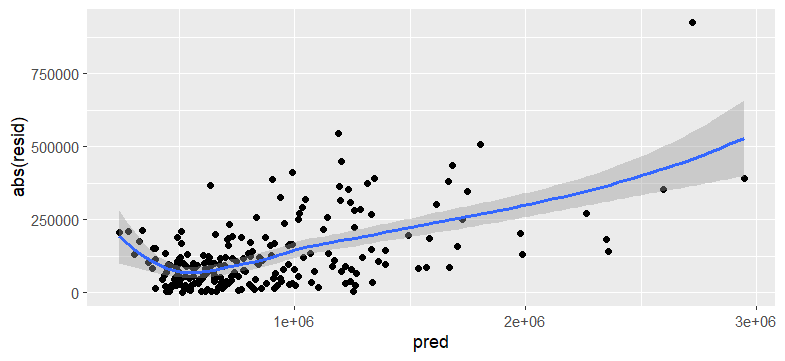
\includegraphics[width=0.8\textwidth]{residual_plot.png}
				\caption{Bubble plot showing influential points.}
			\end{figure}
		\end{columns}
	\end{frame}
	
	\begin{frame}[fragile]{Influence Plot (Bubble Plot) – Identify Influential Values}
		\begin{itemize}
		\end{itemize}
		
		\begin{lstlisting}[language=R, caption=Heteroskedasticity Plot in R]
df <- data.frame(resid = residuals(lm_98105), pred = predict(lm_98105))
ggplot(df, aes(pred, abs(resid))) + geom_point() + geom_smooth()
		\end{lstlisting}
		\begin{lstlisting}[language=Python, caption=Heteroskedasticity Plot in Python]
import seaborn as sns
fig, ax = plt.subplots(figsize=(5, 5))
sns.regplot(model.fittedvalues, np.abs(model.resid), scatter_kws={'alpha': 0.25},
line_kws={'color': 'C1'}, lowess=True, ax=ax)
ax.set_xlabel('predicted')
ax.set_ylabel('abs(residual)')
plt.show()
		\end{lstlisting}
	\end{frame}
	
	\begin{frame}{Histogram of Standardized Residuals: Normality Check}
		\begin{itemize}
			\item \textbf{Purpose:} The histogram assesses residual normality by analyzing the distribution of standardized residuals.
			\item \textbf{Key Insights:}
			\begin{itemize}
				\item Centering Around Zero: The residuals are centered around 0, indicating no strong systematic bias in the model.
				\item Skewness & Long Tails: The right tail is longer, suggesting right-skewness and possible underestimation of some values.
				
				\item Non-Normal Distribution: The residuals deviate from a perfect bell-shaped curve, hinting at potential issues:
					\begin{enumerate}
						\item 	✅ Missing predictors affecting the model.
						\item 	✅ Heteroskedasticity, as observed in the residual plot.
						\item 	✅ Outliers influencing the regression fit.
					\end{enumerate}
			\end{itemize}
		\end{itemize}
	\end{frame}



	\begin{frame}{Histogram of Standardized Residuals: Normality Check}
		\begin{columns}
			
			\column{0.8\textwidth}
			\begin{figure}
				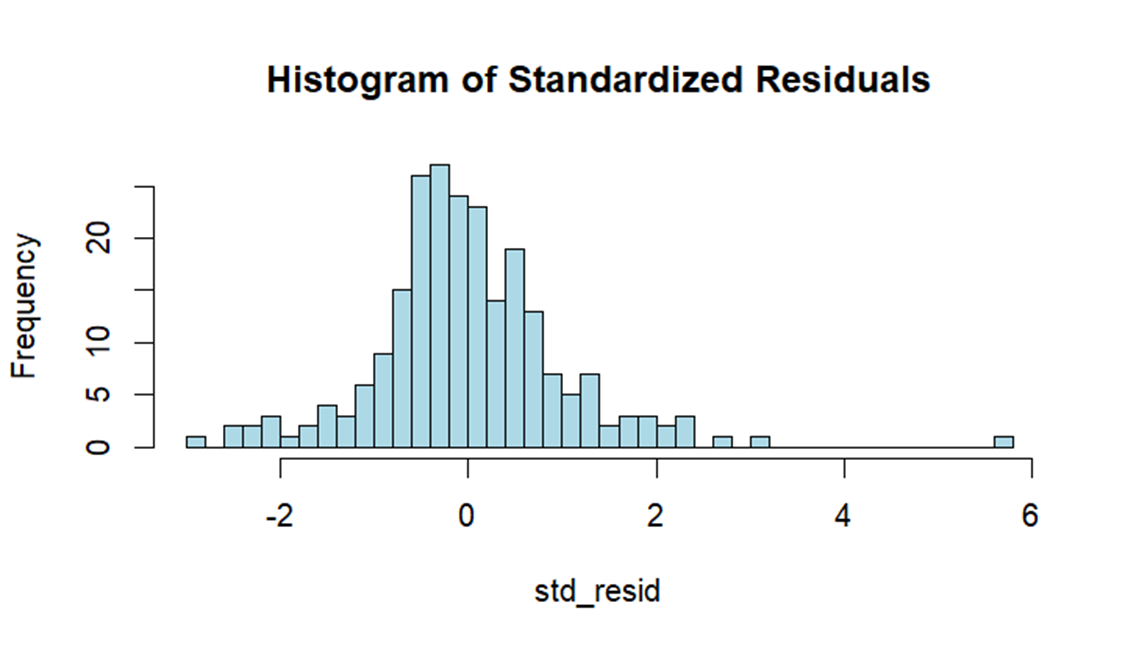
\includegraphics[width=0.8\textwidth]{histo.png}
				\caption{Bubble plot showing influential points.}
			\end{figure}
		\end{columns}
	\end{frame}

\begin{frame}[fragile]{Histogram of Standardized Residuals: Normality Check}
	\begin{itemize}
	\end{itemize}
	
	\begin{lstlisting}[language=R, caption=Histogram of Standardized Residuals in R]
df <- data.frame(resid = residuals(lm_98105), pred = predict(lm_98105))
ggplot(df, aes(pred, abs(resid))) + geom_point() + geom_smooth()
	\end{lstlisting}
	\begin{lstlisting}[language=Python, caption=Histogram of Standardized Residuals in Python]
plt.hist(influence.resid_studentized_internal, bins=50, color='lightblue')
plt.xlabel('Standardized Residuals')
plt.title('Histogram of Standardized Residuals')
plt.show()
	\end{lstlisting}
\end{frame}
	
	% Section 5: Insights & Next Steps
	\section{Insights \& Next Steps}
	
	\begin{frame}{Housing Insights}
		\begin{itemize}
			\item \textbf{Findings}: Linear ties price to size, splines capture nonlinear trends
			\item \textbf{Diagnostics}: Reveal quirks like partial sales—critical for accuracy
			\item \textbf{Application}: Real-world tool for buyers, sellers, and assessors
		\end{itemize}
	\end{frame}
	
	\begin{frame}{Key Takeaways}
		\begin{itemize}
			\item \textbf{Flexible}: Evolves from simple lines to complex curves for housing
			\item \textbf{Precise}: RMSE and cross-validation ensure reliable price predictions
			\item \textbf{Powerful}: R and Python implementations unlock data-driven insights
		\end{itemize}
	\end{frame}
	
	\begin{frame}{Looking Ahead}
		\begin{itemize}
			\item \textbf{Resources}: \textit{Statistical Learning} (Hastie et al.), \textit{Time Series Forecasting} (Shmueli)
			\item \textbf{Next Steps}: Dive into splines, time series for dynamic housing models
			\item \textbf{Call}: Blend theory and practice for smarter predictions
		\end{itemize}
	\end{frame}
	
\end{document}